%
\section{Agent}
Unfortunately, no one can be told what The Agent is. You have to see it for yourself.

\includegraphics[height=5.5cm]{./pics/agent-smith.jpg}
% Why the fuck the first one is ignored?
%-------------------------------------------------------------------
\begin{frame}
\frametitle{Agent history}

\begin{itemize}
%
\item a fork of OCS Inventory UNIX agent by its author
\item started 5 years ago
\item GPLv2
%
\end{itemize}
\end{frame}
%-------------------------------------------------------------------
\begin{frame}

\includegraphics[height=4.0cm]{pics/Perl_Foundation.pdf}
\frametitle{use Perl Luke!}

We choose to use only Perl on the agent side.
\begin{itemize}
\item portable
\item reliable
\item versatil
\end{itemize}
\end{frame}

\begin{frame}
\frametitle{HTTP/HTTPS}
%
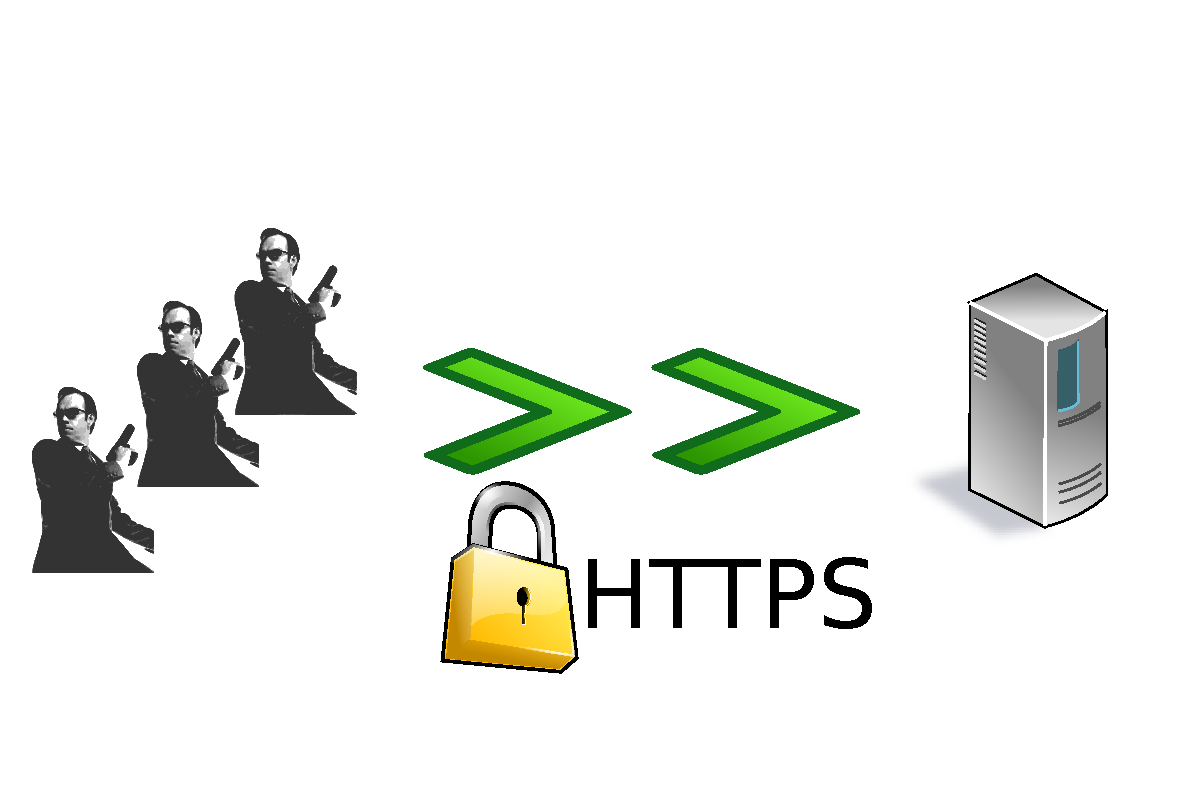
\includegraphics[height=6.0cm]{pics/https.pdf}
%
\end{frame}
\begin{frame}
\frametitle{PUSH/PULL}
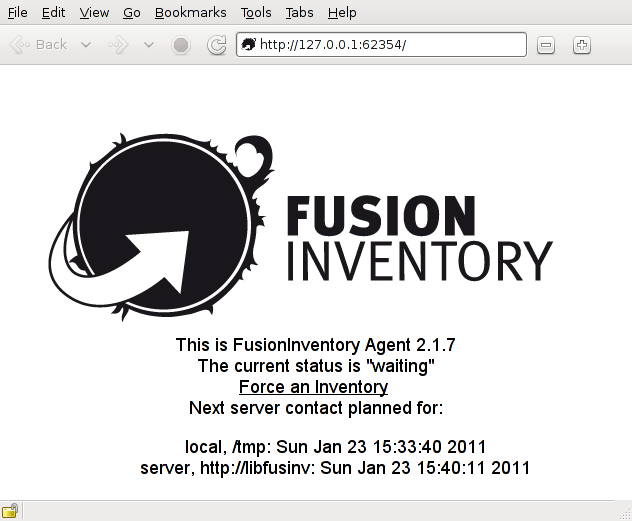
\includegraphics[height=4.0cm]{pics/http-server.png}

thanks to an embedded http server agent get updated by the server or retrieve itself (PULL) request.
%
\end{frame}



\begin{frame}
\frametitle{Task}
%
Not only for local machine inventory. The agent supports different "task".
\end{frame}



\begin{frame}
\frametitle{supported OS (1/2)}
Can run everywhere Perl exist.

\pause
Basicly to do a portage of the agent we
\begin{itemize}
%
\item extend the Inventory modules to collect information
\item and, hum, well, that's all. We're done :D
%
\end{itemize}

\end{frame}
\begin{frame}
\frametitle{supported OS (2/2)}
Supported Operating Systems:
\begin{itemize}
%
\item Linux
\pause
\item BSD
\pause
\item AIX
\pause
\item HP-UX
\pause
\item Solaris
\pause
\item Windows, all from 2000 to Seven 64bit
%
\end{itemize}
\href{http://forge.fusioninventory.org/projects/fusioninventory-agent/wiki/Agent\_supportedplateforms}{A complet list is avalaible on the website.}
\end{frame}
 
